\documentclass{amia}
\usepackage{graphicx}
\usepackage[labelfont=bf]{caption}
\usepackage[superscript,nomove]{cite}
\usepackage{color}
\usepackage{multirow}
\renewcommand*{\thefootnote}{\fnsymbol{footnote}}

\begin{document}

\title{Machine Learning Models for the Segmentation of e-Coaching Text (summarizes the hypothesis of the paper)}

\author{Mehedi Hasan, BS$^{1}$\footnote[1]{Authors provided equal contribution. \label{footnote1}}, Alexander Kotov, PhD$^{1}$\textsuperscript{\ref{footnote1}}, April Idalski Carcone, PhD$^{2}$, Ming Dong, PhD$^{1}$, Sylvie Naar, PhD$^{2}$}

\institutes{
$^1$Department of Computer Science, Wayne State University, Detroit, Michigan \\  
$^2$Department of Family Medicine and Public Health Sciences, School of Medicine, Wayne State University, Detroit, Michigan\\
}

\maketitle

\noindent{\bf Abstract}
\textit{The problem of analyzing temporally ordered observation sequences generated by a physiological, genomic or psychological process to make predictions about the outcome of that process arises in
many domains of clinical informatics.}

1) Motivation: Why do we care about the problem and the results? \\
2) Problem statement: What problem is the paper trying to solve and what is the scope of the work? \\
3) Approach: What was done to solve the problem? \\
4) Results: What is the answer to the problem? \\
5) Conclusions: What implications does the answer imply?

\section*{Introduction}
Temporally ordered sequences of discrete or continuous observations generated by genomic, psychological or psychological processes arise in many different domains of clinical informatics \cite{kotov2015interpretable}\cite{hasan2016study}.

What is the problem? \\

Why is the problem important? \\

What has so far been done on the  problem?\\
1) describes previous work in more technical detail \\
2) as far as needed for a proper understanding of the contribution of the paper \\

What is the contribution of the paper on the problem?\\
1) What are the rival approaches? \\
2) What are the drawbacks of each?\\
3) How has the battle between different approaches progressed?\\
4) What are the major outstanding problems? (This is where you come in)\\

Is the contribution original? Explain why \\

Is the contribution non-trivial? Explain why \\

The authors are not aware of any other work where this approach has been considered.

\section*{Methods}
\subsection*{\textit{Data collection}}
The experimental dataset for this work was constructed from the transcripts of 129 motivational interviews, which include a total of 50,239 segmented and annotated utterances. Each transcript consists
of an MI interview session involving counselor, adolescent, and caregiver. The utterances were annotated based on MYSCOPE codebook \cite{carcone2013provider}, in which the codes are grouped into
patient (adolescent and caregiver) codes and counselor codes. Utterances were divided into successful and unsuccessful communication sequences. Successful communication sequences result in
positive change talk and commitment language statements by an adolescent or caregiver, while unsuccessful sequences are the ones that result in negative change talk or commitment language and the
sequences, in which no change talk or commitment language statements occur. Out of 5143 observed sequences, 4225 were positive and 918 were negative. Successful sequences had an average length of
9.79 utterances, while unsuccessful sequences had on average 9.65 utterances. For each of the probabilistic models (MC and HMM), two models were trained, one model was trained using successful
sequences and another one was trained using unsuccessful sequences. 

Part 1

1) What algorithms or data structures did you select? Who created them? What is their asymptotic behavior? What other specific characteristics are worth noting for this study?\\
2) What programming language and platform did you use? What impact did these choices have on your project?\\


Part 2

1) How specifically did you implement the algorithms?\\
2) How did you handle instrumentation code? Why?\\
3) Did you perform any optimizations? Why or why not?\\
4) How did you choose to test and benchmark your code?\\
5) What inputs (data) did you select to test your implementations? Why?\\

\subsection*{\textit{Segmentation method}}
Generally, a sequence can be viewed as a temporally ordered set of events. In this study, an event is a behavior code that also has a symbolic representation.

\textbf{Naive Bayes}: comming soon...

\textbf{Support Vector Machine}: comming soon...

\textbf{K-Nearest Neighbour}: comming soon...

\textbf{Recurrent Neural Networks}: comming soon...
  
\subsection*{\textit{Evaluation metrics}}
Performance of the proposed method was evaluated in terms of precision, recall, and F-measure using 10 folds cross-validation and weighted macro-averaging of these metrics over the folds. However, LSTM and GRU are trained on 80\% of the data and validated on 10\%. The remaining 10\% of the data is used as a test set for reporting the performance of the model. 

\section*{Results}
Experimental evaluation of the proposed method is conducted on both under and over-sampled sequences. Predictive performance summary of the proposed methods on under and over-sampled sequences is presented in Table.\\

1) In general, the pure, unbiased results should be presented first without interpretation (van Wagenen 1990). \\
2) These results should present the raw data
or the results after applying the techniques outlined in the methods section. The results are simply results; they do not draw conclusions.

\begin{table}[ht]
\centering
\caption{Performance of MC, HMM, and RNN for predicting the success of under and over-sampled patient-provider communication sequences. The highest value for each performance metric is highlighted in bold.}
\label{tab:result_under_over_sampled}
  \begin{tabular}{|l|l|l|l|l|l|l|}
  \hline
   \multirow{2}{*}{\textbf{Method}} & \multicolumn{3}{|c|}{\textbf{lexical features only}} & \multicolumn{3}{|c|}{\textbf{lexical features + topics}} \\\cline{2-7}
   & \textbf{Precision}  & \textbf{Recall} & \textbf{F1-Score} & \textbf{Precision}  & \textbf{Recall} & \textbf{F1-Score}\\ \hline    
    
 Naive Bayes Multinomial & 0.7060 & 0.7044 & 0.7038 & 0.7932 & 0.7799 & 0.7775 \\ \hline
 Support Vector Machine & 0.6395 & 0.6385 & 0.6379 & 0.7111 & 0.7029 & 0.7000\\ \hline
 K-Nearest Neighbour & 0.6244 & 0.6143 & 0.6067 & 0.7775 & 0.7567 & 0.7520\\ \hline
 Long Short Term Memory & \textbf{0.8733} & \textbf{0.8681} & \textbf{0.8677} & \textbf{0.8424} & \textbf{0.8385} & \textbf{0.8381}\\ \hline
 Gated Recurrent Unit & 0.8705 & 0.8676 & 0.8673 & 0.8412 & 0.8377 & 0.8373\\ \hline 
  \end{tabular}
\end{table} 

Predictive performance summary of the proposed methods on under and over-sampled sequences is presented in Table.\\

\begin{table}[ht]
\centering
\caption{Performance of MC, HMM, and RNN for predicting the success of under and over-sampled patient-provider communication sequences. The highest value for each performance metric is highlighted in bold.}
\label{tab:result_under_over_sampled}
  \begin{tabular}{|l|l|l|l|l|l|l|}
  \hline
   \multirow{2}{*}{\textbf{Method}} & \multicolumn{3}{|c|}{\textbf{lexical features only}} & \multicolumn{3}{|c|}{\textbf{lexical features + topics}} \\\cline{2-7}
   & \textbf{Precision}  & \textbf{Recall} & \textbf{F1-Score} & \textbf{Precision}  & \textbf{Recall} & \textbf{F1-Score}\\ \hline    
    
 Naive Bayes Multinomial & 0.7060 & 0.7044 & 0.7038 & 0.7932 & 0.7799 & 0.7775 \\ \hline
 Support Vector Machine & 0.6395 & 0.6385 & 0.6379 & 0.7111 & 0.7029 & 0.7000\\ \hline
 K-Nearest Neighbour & 0.6244 & 0.6143 & 0.6067 & 0.7775 & 0.7567 & 0.7520\\ \hline
 Long Short Term Memory & \textbf{0.8733} & \textbf{0.8681} & \textbf{0.8677} & \textbf{0.8424} & \textbf{0.8385} & \textbf{0.8381}\\ \hline
 Gated Recurrent Unit & 0.8705 & 0.8676 & 0.8673 & 0.8412 & 0.8377 & 0.8373\\ \hline 
  \end{tabular}
\end{table} 

We took the inspiration for the representation of behavior codes from the idea of word embeddings. Word embedding is a representation of words in
low-dimensional space by vectors, which contain the features of the words. In our study, we employed embedding in place of one-hot vectors for representation of behavior codes as input to LSTM and
GRU, since one-hot vectors are high-dimensional and sparse. 

\begin{figure}[!htb]
    \centering
    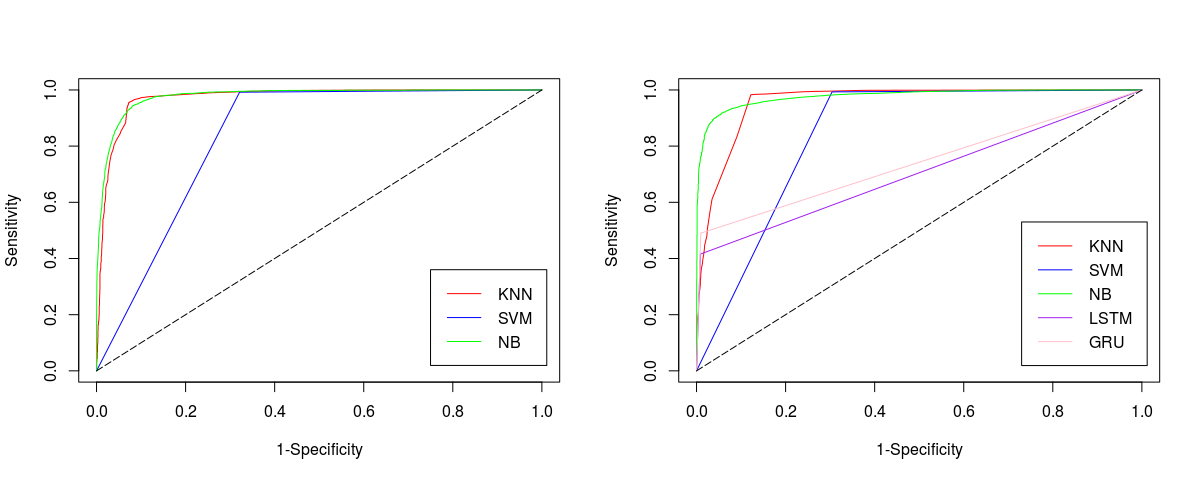
\includegraphics[width=0.90\textwidth]{figures/roc-curves.png}
    \caption{\textbf{ROC curves compared the performance of different models}.}
    \label{fig:roc-curves}
\end{figure}

\section*{Discussion}
By analyzing the experimental results of different communication sequence outcome prediction methods proposed in this paper, we arrived at the following conclusions. First, the overall predictive
performance of RNN models is substantially better than probabilistic models. In particular, the RNN-based method achieves near-human accuracy for predicting the 


1) What, specifically, did you learn from comparing these algorithms or data structures? \\
2) What do your results say about the problem or question you were investigating?\\
3) Was your hypothesis confirmed or disproved?\\
4) Are the results what you expected?\\
5) If you obtained anomalies or other unexpected results, can you explain them? If not, how could you set about in the future to identify what caused them? \\
6) How do your results compare to past findings? Are they consistent? Different?Why? \\
7) How would you respond to objections or questions that other researchers might have about your methods, results, or interpretations? \\
8) What is new and significant?\\
 
\section*{Conclusion}
In this paper, we compared the performance of machine learning models for the task of segmentation of e-coaching text. We found out that k-nearest neighbour provides the best performance for the segmentaion of text in terms of all performance metrics. Manual segmentation of e-coaching data is very resource-intensive and time consuming task, which can significantly decrease the time and effort required to develop effective behavioral interventions. Our
proposed methods can help to identify individual text segments, which can be annotated directly with a classification model and increase
the effectiveness of behavioral interventions. 

1) The hypothesis and the evidence for and against it are briefly restated \\
2) The original motivation is recapitulated \\
3) The state of the field in the light of this new contribution is reassessed \\
4) describes future research and new directions suggested by the contribution\\
5) in particular, research that would improve the evidence for or against the hypothesis

\section*{Acknowledgments}
This study was supported by a grant from the National Institutes of Health, NIDDK R21DK108071, Carcone and Kotov, MPIs. We would like to thank the student assistants in the Department of Family Medicine and Public Health Sciences at Wayne State University School of Medicine for their help in developing the training dataset by manually annotating the dataset using the MYSCOPE codebook. 

\bibliographystyle{vancouver}
\bibliography{References}

\end{document}
